\section{Introduction}

Searches for various BSM theories including SUSY have been performed at LHC  alongside searching for the Higgs and performing different SM anlyses. Many SUSY searches were conducted targeting the production of squarks and gluinos. This was motivated by a larger theoretical cross-section and therefore higher probability of producing coloured superpartners \cite{borschensky2014squark}. Up to this moment no statistically significant excess over SM has been detected and exclusion limits were placed on masses of SUSY particles. Figure~\ref{fig:SUSYlimit} shows the latest data on the masses that have been excluded for supersymmetric particles in various production scenarios. The lower limits on the masses of most squarks and gluinos in different searches significantly exceed 1 TeV \citep{aad2015summary}. As a consequence, if their production occurs, it is either extremely rare at present energies or requires higher energy of collision to leave an identifiable signature. 

This thesis's research will focus on the electroweak production as one of the possible SUSY particle production scenario. Sleptons and gauginos are produced in electroweak production processes and are not affected by the strong force. They have smaller cross-sections compared to squarks and gluinos, so their theoretical production rate is smaller. However, if their masses are small compared to the strongly interacting sparticles, SUSY production will likely be dominated by electroweak production where sparticles have smaller mass and current energy might be enough to produce them in quantities that would allow their detection \citep{atlas2015search}. 
%\newgeometry{left=1cm,right=1cm}
\begin{figure}[!ht]
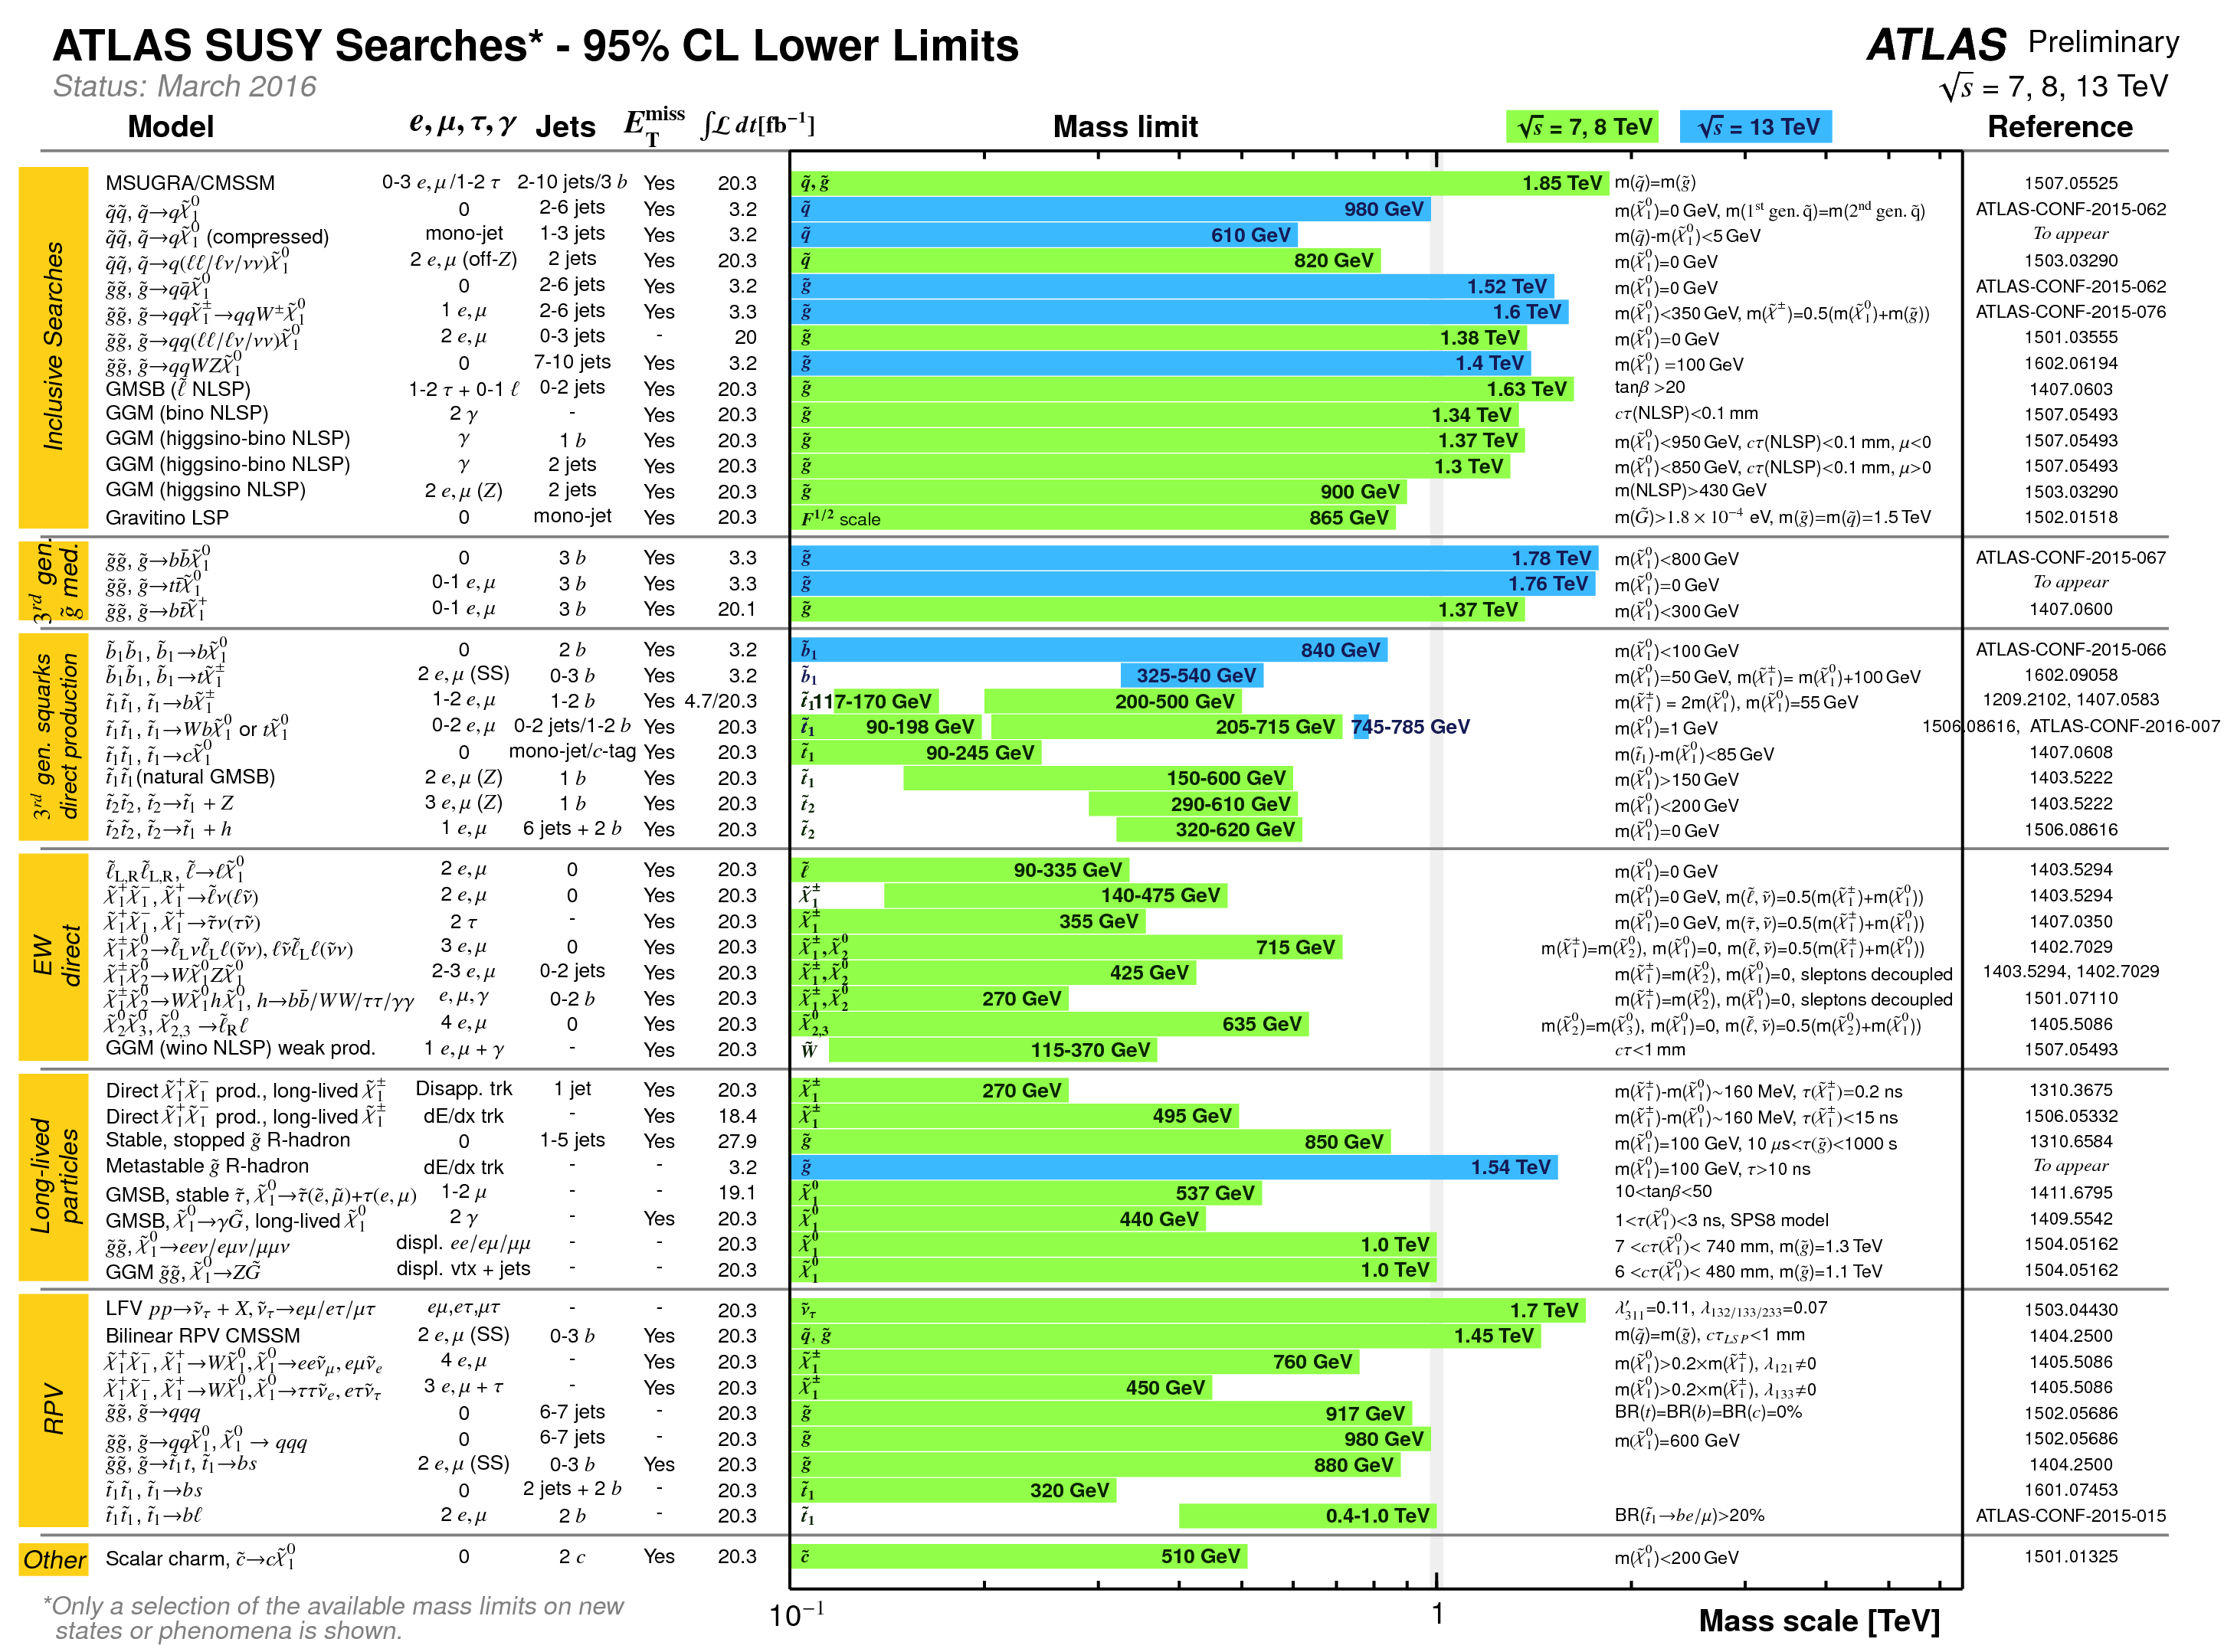
\includegraphics[width=\textwidth]{Chap3/ATLAS_SUSY_Summary.png}
\caption[Exclusion limits of ATLAS searches for Supersymmetry]{Exclusion limits of ATLAS searches for Supersymmetry \citep{SUSYlimits}}
\label{fig:SUSYlimit}
\end{figure}
\cleardoublepage


So far searches in the electroweak region have been unable to find evidence of supersymmetric particles. Limits on their masses according to various decay scenarios have been obtained and can be seen in Fig \ref{fig:summaryplot}.
\begin{figure}[!ht]
	\centering
	\captionsetup{width=0.8\textwidth}
	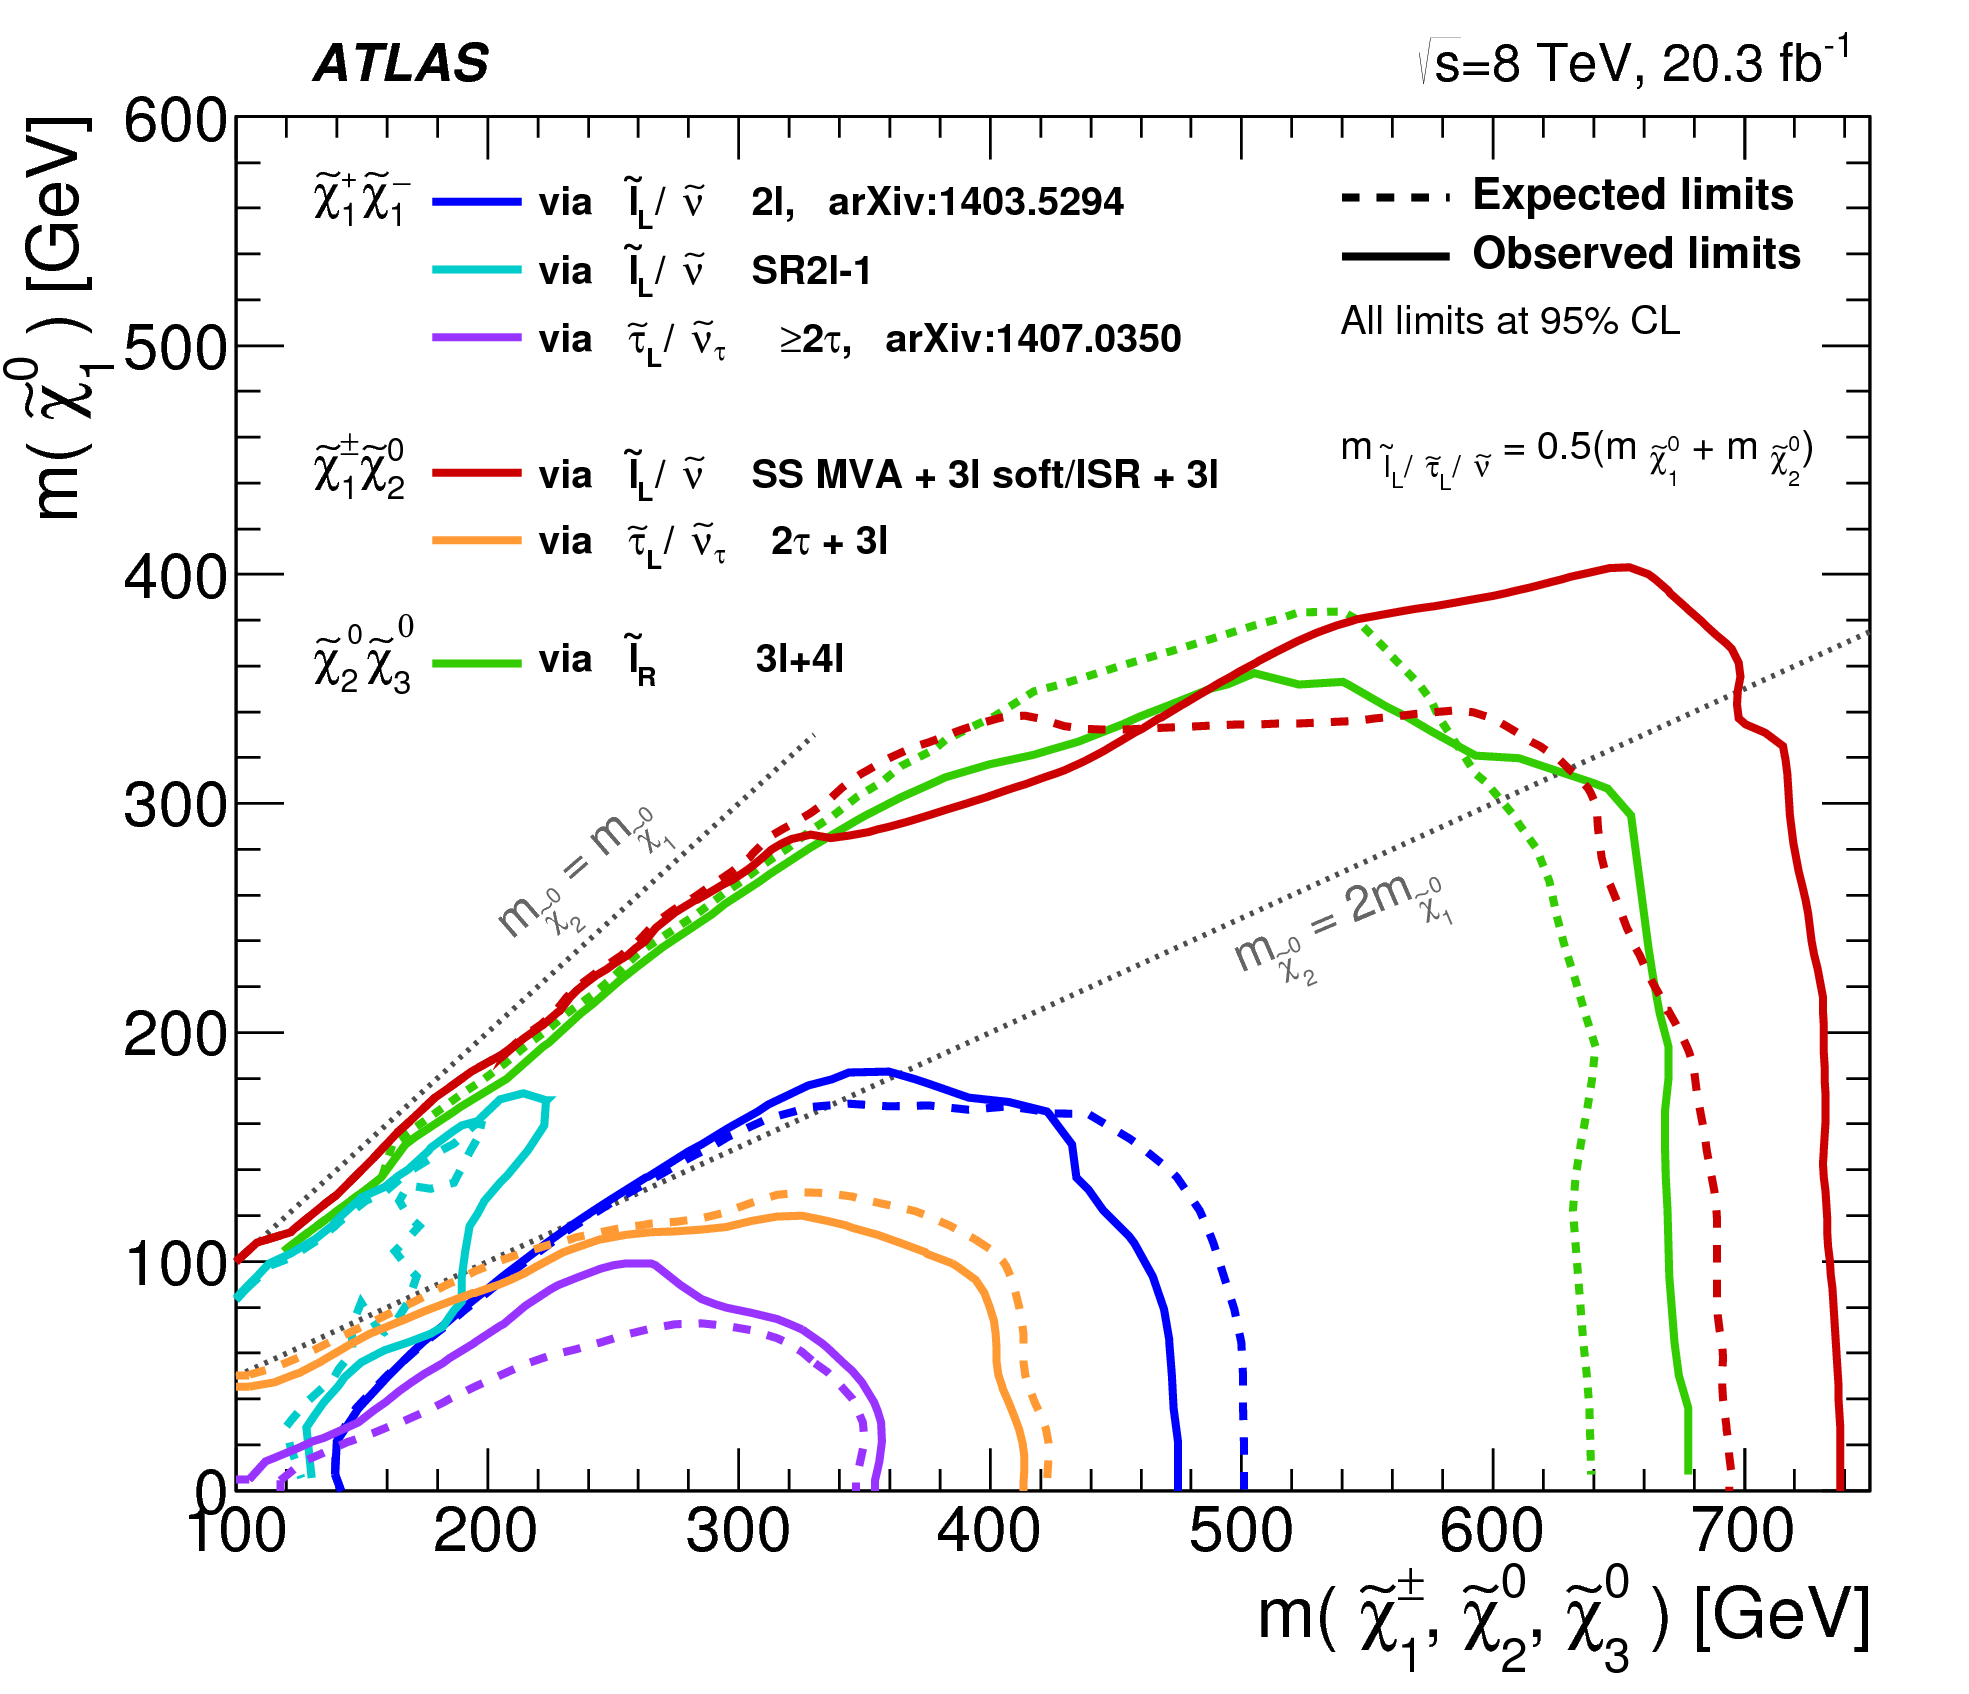
\includegraphics[scale=0.15]{Chap3/fig_19b}
	\caption[Exlcusion limits on electroweak production at ATLAS]{The 95\% CL exclusion limits on $\chi_1^+\chi_1^-$, $\chi_1^{\pm}\chi_2^0$ and $\chi_2^0\chi_3^0$ production with $l$-mediated decays, as a function of the $\chi_1^{\pm},\,\chi_2^0$ and $\chi_1^0$ masses \citep{aad2016search}. }\label{fig:summaryplot}
\end{figure}

These results are taken from \citep{atlas2015search} analysis performed at $\sqrt{s}=$8 TeV and integrated luminosity of 20.3 fb\textsuperscript{-1}. The search was performed based on various scenarios of the pMSSM, involving electroweak production of charginos and neutralinos. The turquoise and blue lines represent decay scenarios that are relevant for this paper as they show information on slepton-mediated decays of a chargino pair. 
In particular, the production of $\tilde{\chi}^{+}_{1}\tilde{\chi}^{-}_{1}$ pair decaying through a slepton ($\tilde{\ell}$) with final states contatining two opposite sign leptons will be considered (see Fig. \ref{fig:EWchargino}). 
\begin{figure}[!h]
  \centering   	
  	\captionsetup{width=0.8\textwidth}
	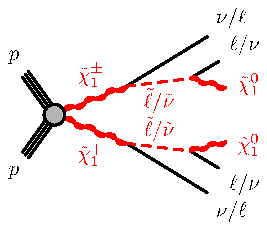
\includegraphics[]{Chap2/C1C1-llvvN1N1-slsnu}	
\caption[Feynman diagram of slepton-mediated chargino decay]{Electroweak chargino pair production in proton-proton collisions with intermediate slepton in the decay process.}\label{fig:EWchargino}
\end{figure}  

In the nomenclature used at LHC and in this thesis, electrons and muons are called "light leptons". Taus are considered separately as they decay very promptly and therefore are very difficult to reconstruct. This thesis only focuses on final states containing electrons and muons and thus the designation "lepton" only refers to these particles.  


%However, given that so far only 3.2 fb\textsuperscript{-1} of integrated luminosity has been achieved at $\sqrt{s} = 13$ TeV.

\subsection{Overview of search methods}
Detecting new physics events at LHC requires using computational and statistical methods that can deal with the type of information a particle accelerator produces. The data is initially collected using triggers corresponding to the type of events under analysis. Each event has a large number of physical characteristics such as momentum, energy, mass, multiplicities, etc. The numbers representing them are all stored in a data structure which then can be accessed, modified and analysed using software tools. 

The cornerstone of all accelerator physics analyses is the correct estimation of background events. All background events represent physics that is already known and that has some similar or identical features with the processes we wish to study. For instance, this thesis focusses on the reactions that have precisely two oppositely charged leptons in their final states. A number of processes well described by the standard model share this characteristic and therefore will form the background. 

The task of correctly identifying background is therefore crucial in the process of searches for new physics events. Monte Carlo (MC) simulations are used to generate background events distribution samples according to a probability density function of a particular process. In this thesis MC simulated data samples are used to model SM background events along with SUSY signal events. All the samples include events that can result in dileptonic decays. 

The data is then overlaid on the simulated background to see whether there is a disagreement between data and background. If there is a significantly large excess of data over background it can lead to new discoveries such as existence of a new particle.  The presence of a new particle can reveal itself in a number of ways. The easiest case to detect is finding an abnormality in mass distribution, as was the case with the discovery of the Higgs. The narrow peak over a smooth line in mass distribution of diphoton events constituted a significant excess over SM predictions and was in agreement with theoretical predictions \citep{chatrchyan2012observation,Aad:2012tfa}. 

\begin{figure}
	\centering
	\captionsetup{width=0.8\textwidth}
	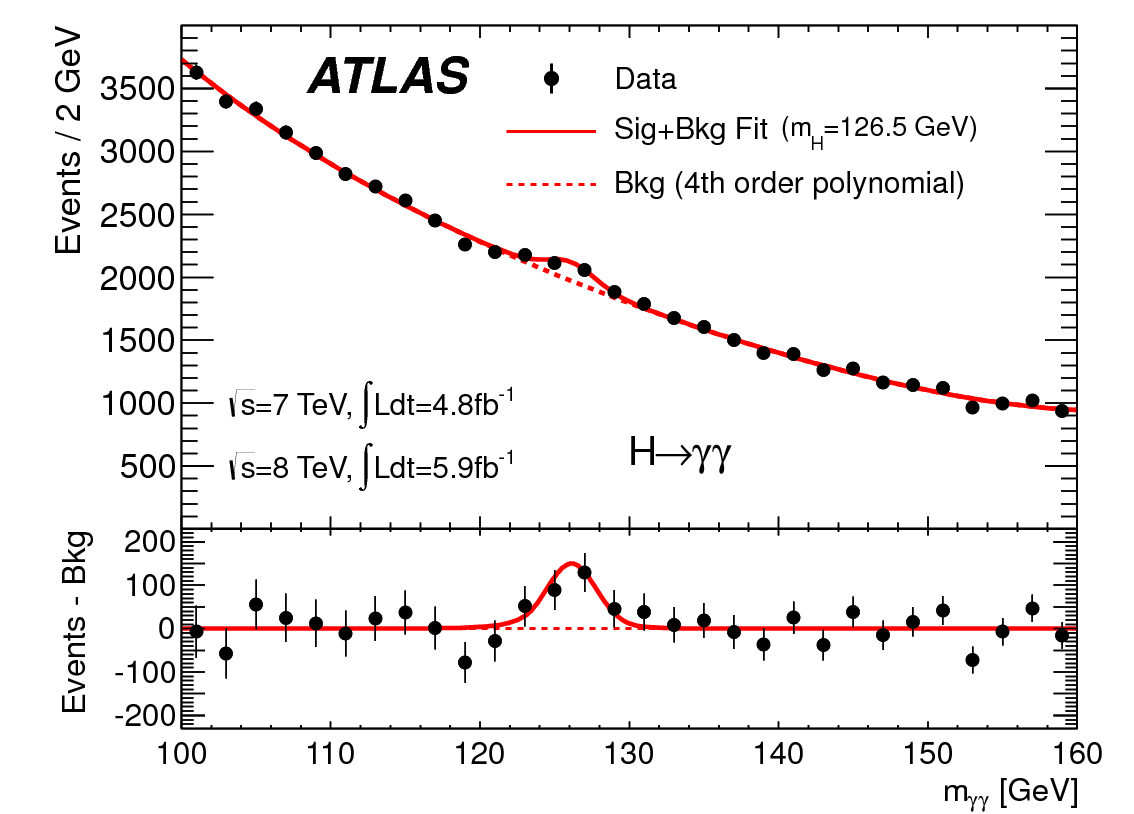
\includegraphics[scale=0.2]{Chap3/figaux_004a}
	\caption[Invariant mass of diphoton events: discovery of the Higgs]{Invariant mass distribution of diphoton 				candidates for the combined $\sqrt{s}$ = 7 TeV and $\sqrt{s}$ = 8 TeV 			data samples. The mass of the Higgs corresponds to the peak at 126.5 				GeV \citep{Aad:2012tfa}.}
\end{figure}

Unfortunately, this method does not work well for SUSY particles and other techniques have to be used. Standard search techniques involve defining \textbf{signal regions} in data distributions that are sensitive to possible SUSY signals and looking whether there is a significant excess over SM background predictions in these regions. 
This also includes looking for abnormal tails in distributions of different variables that are not in agreement with SM predictions. These variables will be discussed in the subsection \ref{subsec:Variables}. Signal regions are usually determined using cut-and-count approach that will be discussed in the subsection \ref{subsec:stat}.

\subsection{Event selection}

Event reconstruction is the process of turning raw data into manageable format that includes quantities needed in physics analysis. An event has to pass certain identification criteria to be chosen for reconstruction. Correct identification of different physics objects at LHC includes a large number of dedicated algorithms not presented in this thesis, but are available elsewhere \citep{Aad:2016tuk}. 
However, in this section a very general outline of the selection procedure for reactions that result in two leptonic decays will be given. All "signal" objects have to pass a set of criteria to obtain a high quality sample with minimum possible contamination.

Signal electrons are required to have $|\eta|<2.47$ and transverse momentum $p_{T}>10$ GeV. These are inferred from the calibrated  energy deposits in the EmCal and must have a matching ID track. Signal muons are reconstructed using information from MS and ID tracks and are required to have   $|\eta|<2.5$ and $p_{T}>10$ GeV. Jets are reconstructed using information from calorimeters and are divided into "central" and "forward" categories. Central jets must have $|\eta|<2.4$ and $p_{T}>20$ GeV. Forward jets are those with $2.4<|\eta|<4.5$ and $p_{T}>30$ GeV. 

One of the common techniques used in LHC analyses is the identification of central jets that have $b$-hadrons (hadrons containing bottom quark/s).  These jets are referred to as $b$-tagged and are identified using multivariate techniques based on machine learning instruments such as artificial neural networks and boosted decision trees \citep{Aad:2015ydr}. The efficiency of $b$-tagging has been significantly improved in run-II due to the addition of the Insertable B-Layer in the ID. $b$-tagging is an extremely useful technique because some important heavy particles such as top quark and the Higgs decay into bottom quarks. 

\subsection{Event variables used in the analysis}
\label{subsec:Variables}

A set of discriminating variables associated with searches for evidence of SUSY is presented here. Topological and kinematic variables as well as quantities derived from them will be investigated.

\begin{itemize}[leftmargin=0cm]
\item[]$\bm{p^X_T}$ The transverse momentum of an object $X$.
\item[]$\bm{\Delta\phi(X,Y)}$ The separation between two reconstructed objects $X$ and $Y$, e.g. $\bm{\Delta\phi(E_T^{miss},\ell)}$.
\item[]$\bm{E^{miss}_{T}}$ The magnitude of the missing transverse momentum of the event. Missing transverse momentum is defined as the negative of the sum of all reconstructed objects' transverse momenta.
\item[]$\bm{E^{miss,rel}_T}$ This value is defined as 
\[
 E_T^{miss,rel} = 
  \begin{cases} 
   E_T ^{miss}\quad & \text{if } \Delta\phi(E_T^{miss},\ell/j) \geq \pi/2 \\
   E^{miss}_T\times \text{sin}\Delta\phi(E^{miss}_T,\ell/j) \quad      & \text{if } \Delta\phi(E^{miss}_T,\ell/j)<\pi/2
  \end{cases}
\]
\hspace{1cm} where $\Delta\phi(E_T^{miss},\ell/j)$ is the azimuthal angle between the direction of $E_T^{miss,rel}$ 
\hspace{1cm} and that of the nearest electron, muon, or central jet. 
\item[]$\bm{p_{T,ll}}$ The transverse momentum of the two-lepton system. 
\item[]$\bm{m_{ll}}$ The invariant mass ow two leptons.
\end{itemize}

Another derived variable is $\bm{m_{T2}}$ called "stransverse mass". It was introduced as a way to infer information about undetected particles and is also useful in suppressing background. It is used to put bound the masses of unseen particles

is an event variable used to bound the masses of an unseen pair of particles which are presumed to have decayed semi-invisibly into particles which were seen. MT2 is therefore a function of the momenta of two visible particles and the missing transverse momentum in an event


\subsection{Cut-and-count approach and test statistics}
\label{subsec:stat}
As was discussed previously a good signal region retains as many signal events as possible while at the same time cutting off background events. The way to suppress the background is to use successive cuts. The cuts are based on determining physical quantities that are able to discriminate between signal and background. The choice for a single cut is motivated both by theoretical considerations and the shape of the MC   signal and background distributions. 

To optimize a cut or a set of cuts a metric that shows the discriminating power is needed. The numerical expression of how well a cut performs is given by a score function and its result will be referred to as "significance". The score function is constructed in the following way.
The total number of events in a particular selection $N$, and it is the sum of $S$ and $B$, which refer to the number of signal and background events respectively. And this gives
\begin{equation}
S = N -B
\end{equation}
The uncertainty of $S$ is then
\begin{equation}
\sigma^2(S) = \sigma^2(N) + \sigma^2(B) = N+\sigma^2(B)
\end{equation}
 

The concept of p-value is very important in determining how significant a certain event is. A basic statistical test assumes two hypotheses - null hypothesis, stating that there is no significant excess, and alternative hypothesis, stating the opposite.
To demonstrate it the standard normal distribution will be used. 
 
